\documentclass[14pt]{extarticle}

\usepackage[english]{babel}
\usepackage[utf8]{inputenc}
\usepackage{hyperref}
\usepackage{graphicx,eso-pic}
\usepackage{newtxtext}
\usepackage{setspace}
\usepackage{multirow}
\usepackage{array}
\usepackage{lipsum}
\usepackage{titlesec}
\usepackage{multicol}
\usepackage{pdfpages}
\usepackage{indentfirst}
\usepackage[bottom=1.5cm,top=2.5cm,left=2cm,right=2cm]{geometry}

\hypersetup{
    colorlinks=true,
    linkcolor=black,
    filecolor=magenta,
    urlcolor=blue,
    pdftitle={Synopsis},
    pdfpagemode=FullScreen,
    }

\urlstyle{same}

\makeatletter

\setlength{\parskip}{1em}

\newcommand\frontmatter{
    \cleardoublepage
    \pagenumbering{roman}
}

\newcommand\mainmatter{
    \cleardoublepage
    \pagenumbering{arabic}
}

\newcommand\backmatter{
    \if @openright
        \cleardoublepage
    \else
        \clearpage
    \fi
}

\makeatother

\titleformat{\section}[block]{\Large\bfseries\filcenter}{}{1em}{}


\title{}
\author{}
\date{}

\begin{document}

\frontmatter

\newgeometry{bottom=2cm,top=2cm,left=1.5cm,right=1.5cm}
\addcontentsline{toc}{section}{Title}
\vspace{-7em}
\maketitle

\vspace{-7em}

\begin{center}
    \singlespacing
\textbf {A Project Work Synopsis} \\

\vspace{1cm}
\onehalfspacing
\emph {Submitted in partial fulfilment for the award of the degree of} \\

\vspace{1.5cm}
\singlespacing

\textbf{
BACHELOR OF ENGINEERING \\
IN \\
COMPUTER SCIENCE and ENGINEERING - INTERNET of THINGS\\
}

\vspace{2.5em}
\onehalfspacing
\textbf{
Submitted by : \\
\begin{tabular}{ccccc}
    Rishabh Anand & Abhishek Singh & Shefali Yadav \\
    19BCS4525 & 19BCS4508 & 19BCS4524 \\
\end{tabular}
}

\textbf{
Under the Supervision of : \\
Nikhil Aggarwal
}

\vspace{1em}

\includegraphics[scale=0.25]{private/seal.png}

\singlespacing

CHANDIGARH UNIVERSITY, GHARUAN, MOHALI - 140413\\
Punjab

\onehalfspacing
August, 2021

\end{center}
\restoregeometry


\newpage
\addcontentsline{toc}{section}{Acknowlgement}
\section*{Acknowlgement}

We, 'Rishabh Anand', 'Abhishek Singh' and 'Shefali Yadav', students of 'Bachelor of Engineering in Computer Science and Engineering - IoT', session:2019-23, Department of Computer Science and Engineering, Apex Institute of Technology, Chandigarh University, Punjab, hereby declare that the work presented in this Project Work entitled 'Federated Learning With IoT Devices' is the outcome of our own bona fide work and is correct to the best of our knowledge and this work has been undertaken taking care of Engineering Ethics. It contains no material previously published or written by another person nor material which has been accepted for the award of any other degree or diploma of the university or other institute of higher learning, except where due acknowledgment has been made in the text.

\vspace{5em}
\begin{flushright}
    Rishabh Anand\\
    19BCS4525
\end{flushright}

\vspace{13em}
Date: 08 April, 2022 \\

Place: Ludhiana (Punjab)\\

\newpage

% \newpage
% \addcontentsline{toc}{section}{Timeline}

% \section*{Timeline}
% \begin{center}
%     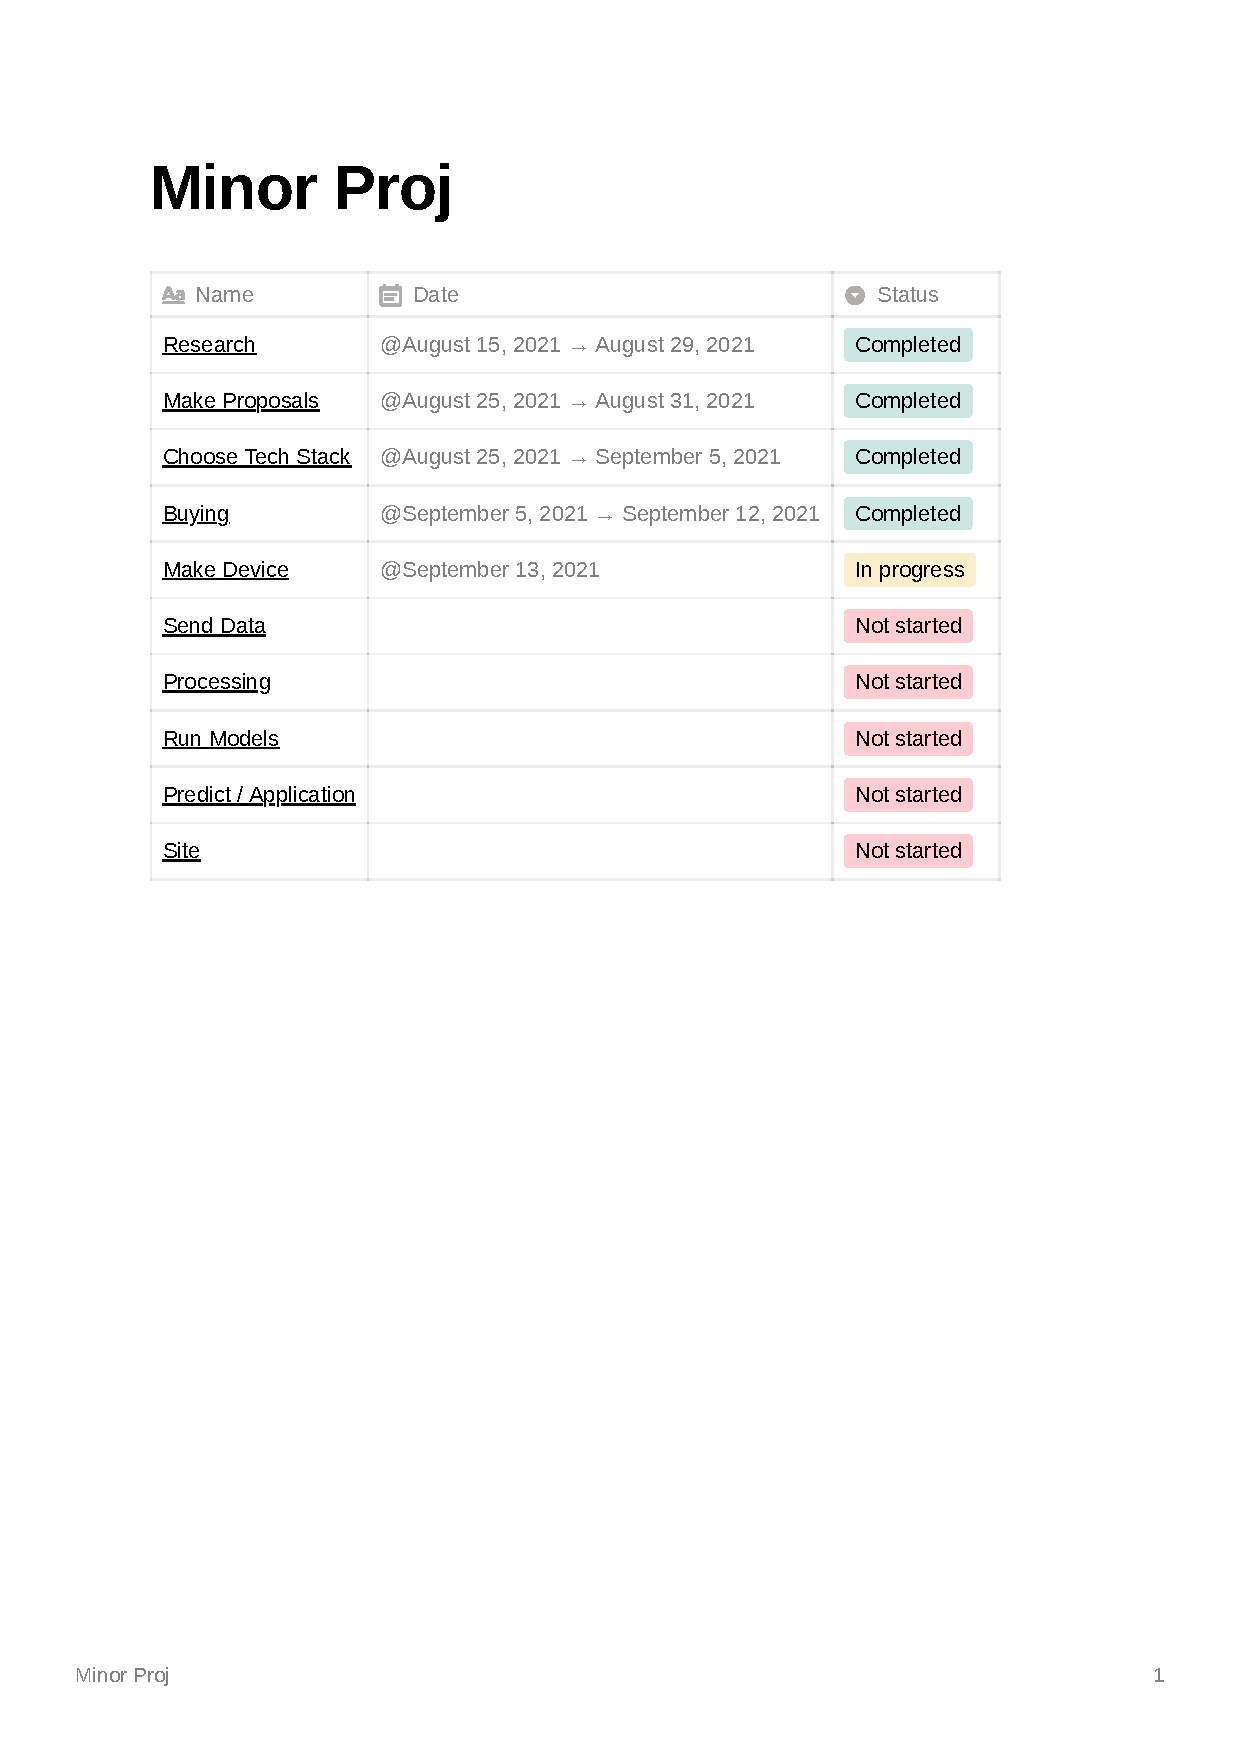
\includegraphics[width=.75\textwidth]{private/gantt.png}
%     \includegraphics[width=.75\textwidth]{private/gantt2.png}
% \end{center}


% \newpage
% \addcontentsline{toc}{section}{List of figures}
% \listoffigures

% \newpage
% \addcontentsline{toc}{section}{List of tables}
% \listoftables

\setlength{\parskip}{0em}
\newpage
\addcontentsline{toc}{section}{CONTENTS}
\begin{center}
    \tableofcontents
\end{center}

\mainmatter

\setlength{\parskip}{1em}

\newpage
\section{INTRODUCTION}
% \subsection{Project Definition}

\par In a world, divided by fear, of losing your loved ones, of losing your loved belongings,of losing your life, we hope to come up with a solution that should keep you and your dreams safe. Because that's what EarthQuake's take away... Even after the major tremor, what hurts more is the AfterShocks that follow. These are produced by the stress that was caused by the earthquake.

\par This project gives us a second chance at saving lives by using Artificial Intelligenceto determine where the next tremor is going to be. So that you can move, and get to asafer place. Methods like Columnb's Stress Criterion are being used in current times toexplain the spatial distributions of AfterShocks, but as the advent of science \& technologyis improving, we hope to introduce Machine Learning models that can find an undiscoveredpattern which will be helpful in predicting the fair locations of AfterShocks.

\par Once we have our predictions, it is very important to display them in a good manner sothat Uncle Bob can understand them and move himself to safety. We have created a Reactweb-app just for this purpose so that it is easily acessible to people and move them fromharm's way. Thereby, reducing the damage to both people and resources, thus, makingthis world a better place.

% \newpage
% \subsection{Project Overview}

% \par TBD

\newpage
\section{LITERATURE SURVEY}
\subsection{Existing System}

\subsubsection{Coulomb failure stress change :}
\par In this we  use a deep-learning approach to identify a static-stress-based criterion that forecasts aftershock locations without prior assumptions about fault orientation. We show that a neural network trained on more than 131,000 mainshock-aftershock pairs can predict the locations of aftershocks in an independent test dataset of more than 30,000 mainshock-aftershock pairs more accurately (area under curve of 0.849) than can classic Coulomb failure stress change (area under curve of 0.583). We find that the learned aftershock pattern is physically interpretable: the maximum change in shear stress, the von Mises yield criterion (a scaled version of the second invariant of the deviatoric stress-change tensor) and the sum of the absolute values of the independent components of the stress-change tensor each explain more than 98 per cent of the variance in the neural-network prediction. This machine-learning driven insight provides improved forecasts of aftershock locations and identifies physical quantities that may control earthquake.

\subsubsection{Research by harvand and google machine learning experts}
\par They  started with a databse of information on more than 118 major earthquakes from around the world.From there, they applied a neural network to analyze the relationships between static stress changes caused by the mainshocks and aftershock locations. The algorithm was able to identify useful patterns.
\par The end result was an improved model to forecast aftershock locations and while this system is still imprecise, it's a motivating step forward. Machine learning-based forecasts may one day help deploy emergency services and inform evacuation plans for areas at risk of an aftershock.When they applied neural networks to the data set, they were able to look under the hood at the specific combinations of factors that it found important and useful for that forecast, rather than just taking the forecasted results at face value. This opens up new possibilities for finding potential physical theories that may allow us to better understand natural phenomena.


% \newpage
% \subsection{Proposed System}



% \par TBD

% \newpage
% \subsubsection{Comparision of Various Framworks}

% \newpage
% \section{PROBLEM FORMULATION}

% \par TBD

% \newpage
% \section{RESEARCH OBJECTIVES}

% \par TBD

% \newpage
% \subsection{The Steps}

% \newpage
% \subsection{Challanges }

\newpage
\section{METHODOLOGY}

\par The idea is to observe a volume which extends 100 km horizontally and 50 km vertically from the main shock. We then break that volume into 5kmx 5km x 5km small volumes and calculate the elastic stress change tensors at each of their centroid.
\par Now using that information we need to predict whether there was an aftershock in that small volume or not. In order to know the ground truth we use International Seismological Center(ISC) event catalogue, in which for each main shock we looked up for its corresponding aftershocks from 1 sec to 1 year time and using that information we created our ground truth i.e. whether there was an aftershock in that small volume or not.
\par So this whole problem is now a binary classification problem, in which our neural network has to predict was there an aftershock in that small 5km x 5km x 5km region or not. The model will use deep learning techniques to predict whether there can be aftershock at a particular locations or not. I'll be taking the data providedby the SRCMOD http://equake-rc.info/SRCMOD/searchmodels/allevents/.
\par The format of the data will be FSP (finite-source rupture model). We'll not be working on how to process those SRCMOD files in order to create a csv. Rather we'll use already created CSVs.
\par The data provided by the SCRMOD file contains the information about the hypocenter, latitude, longitude, magnitude, strike, dip, the inversion parameters and many other relevant data that is sufficient to get an insight of the earthquake.
\par We'll be feeding these data to the neural network having several hidden layers (it depends on you, try and experiment with it), which will then try to extract the important features in order to predict the whether there is a chance of having an aftershock or not. we'll be using two activation functions tanh and ReLu (again experiment with it). The output layer will be a sigmoid layer, which will give us a probability between 0 - 1, as to how confident it is.


\backmatter

\newpage
\addcontentsline{toc}{section}{TENTATIVE CHAPTER PLAN}
\section*{TENTATIVE CHAPTER PLAN}

\textbf{CHAPTER 1: INTRODUCTION }

\par This chapter introduces the reader to Federated learning and the basics of the project.

\textbf{CHAPTER 2: LITERATURE SURVEY}

\par This chapter includes the research already available for Applying Federated learning. The findings of the researchers will be highlighted which will become the basis of current implementation. And the existing and current approaches are compared.

\textbf{CHAPTER 3: PROBLEM FORULATION}

\par This chapter covers the basic problem formulations and defines the solution as provided by the paper.

\textbf{CHAPTER 4: RESEARCH OBJECTIVES}

\par This chapter covers the main differences between distributed learning and federated learning. Also, it includes the steps and the challenges of federated learning, how we can use it and how we can overcome the challenges.

\textbf{CHAPTER 5: METHODOLOGY}

\par This chapter covers the technical details of the proposed approach.

\textbf{REFERENCES}

\par This Section contains the references to other documents that are either useful or are directly reffered in this article.


\newpage
\addcontentsline{toc}{section}{REFERENCES}
\section*{REFERENCES}
\begin{enumerate}
    \item https://www.blog.google/technology/ai/forecasting-earthquake-aftershock-locations-ai-assisted-science/
    \item https://www.nature.com/articles/s41586-018-0438-y\#author-information
    \item Båth, M. Lateral inhomogeneities of the upper mantle. Tectonophysics 2, 483-514 (1965).
    \item Utsu, T. A statistical study on the occurrence of aftershocks. Geophys. Mag. 30, 521-605 (1961).
    \item Parsons, T., Stein, R. S., Simpson, R. W. \& Reasenberg, P. A. Stress sensitivity of fault seismicity: a comparison between limited-offset oblique and major strike-slip faults. J. Geophys. Res. 104, 20183-20202 (1999).



\end{enumerate}

\end{document}